%page1
\begin{figure}
  \begin{subfigure}[b]{0.33\linewidth}
    \centering
    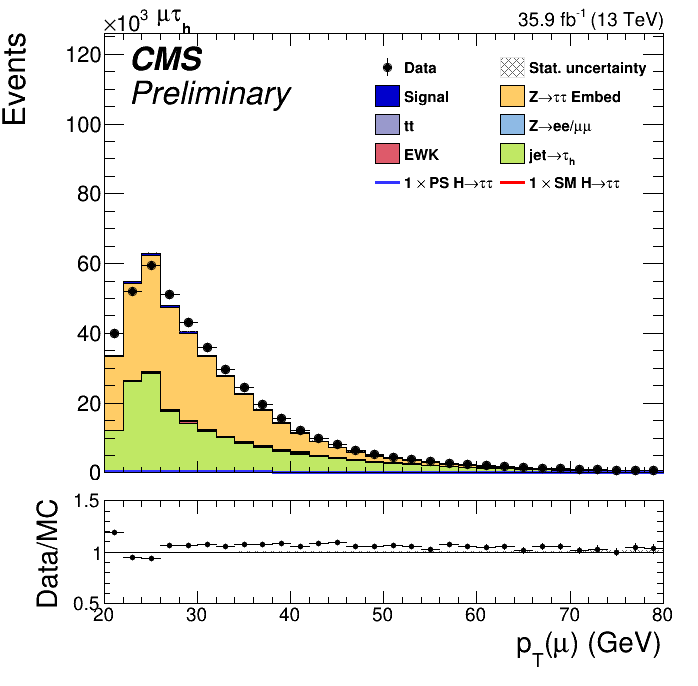
\includegraphics[width=\linewidth]{Chapitre7/Images/CtrlPlots/2016/MuonpT.png} 
    \caption{$p^{\mu}_T$, 2016.} 
    \vspace{0.5ex}
  \end{subfigure}%% 
  \begin{subfigure}[b]{0.33\linewidth}
    \centering
    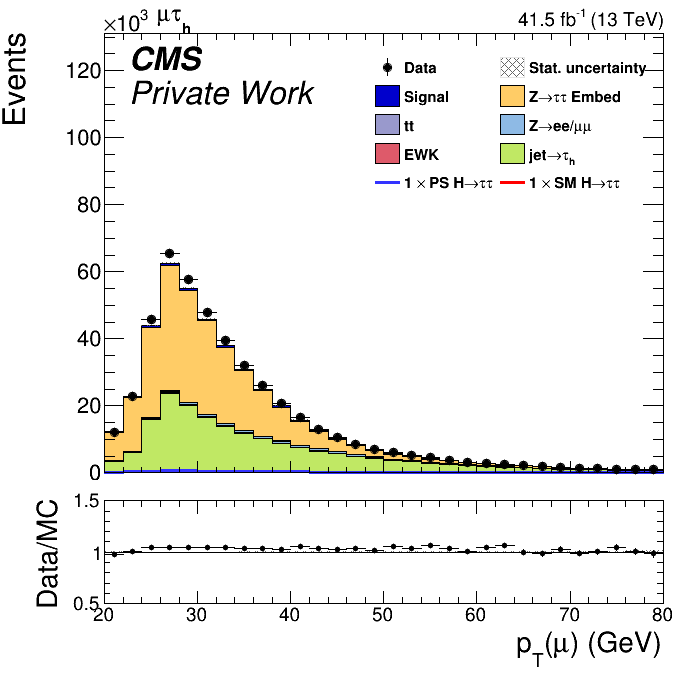
\includegraphics[width=\linewidth]{Chapitre7/Images/CtrlPlots/2017/MuonpT.png} 
    \caption{$p^{\mu}_T$, 2017.} 
    \vspace{0.5ex}
  \end{subfigure} 
    \begin{subfigure}[b]{0.33\linewidth}
    \centering
    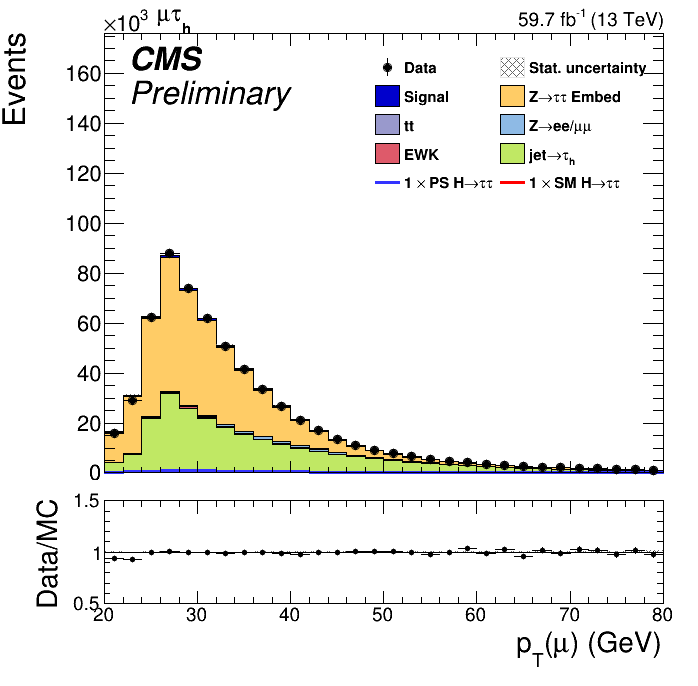
\includegraphics[width=\linewidth]{Chapitre7/Images/CtrlPlots/2018/MuonpT.png} 
    \caption{$p^{\mu}_T$, 2018.} 
    \vspace{0.5ex}
  \end{subfigure} 

    \begin{subfigure}[b]{0.33\linewidth}
    \centering
    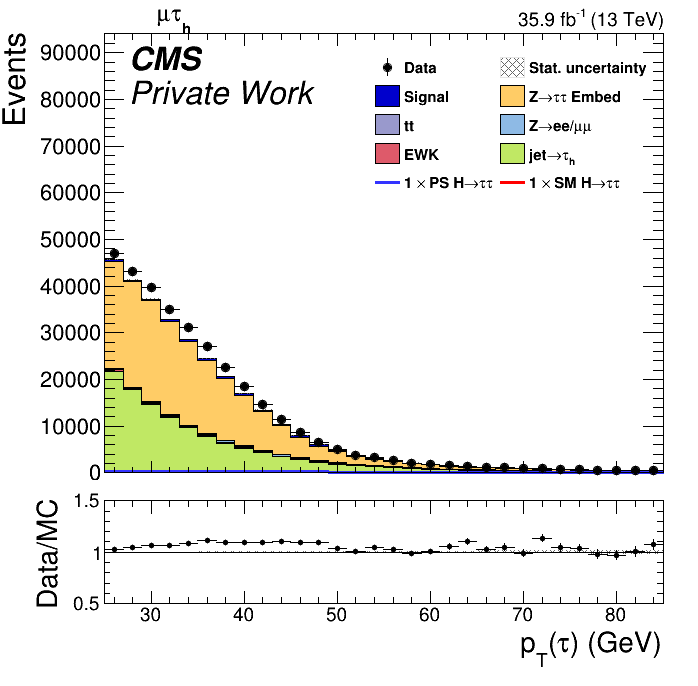
\includegraphics[width=\linewidth]{Chapitre7/Images/CtrlPlots/2016/TaupT.png} 
    \caption{$p^{\tau_h}_T$, 2016.} 
    \vspace{0.5ex}
  \end{subfigure}%% 
  \begin{subfigure}[b]{0.33\linewidth}
    \centering
    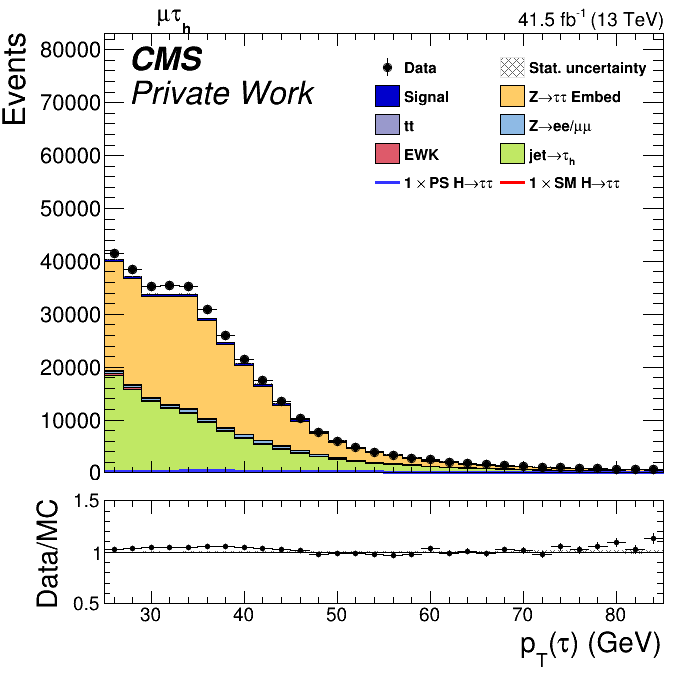
\includegraphics[width=\linewidth]{Chapitre7/Images/CtrlPlots/2017/TaupT.png} 
    \caption{$p^{\tau_h}_T$, 2017.} 
    \vspace{0.5ex}
  \end{subfigure} 
    \begin{subfigure}[b]{0.33\linewidth}
    \centering
    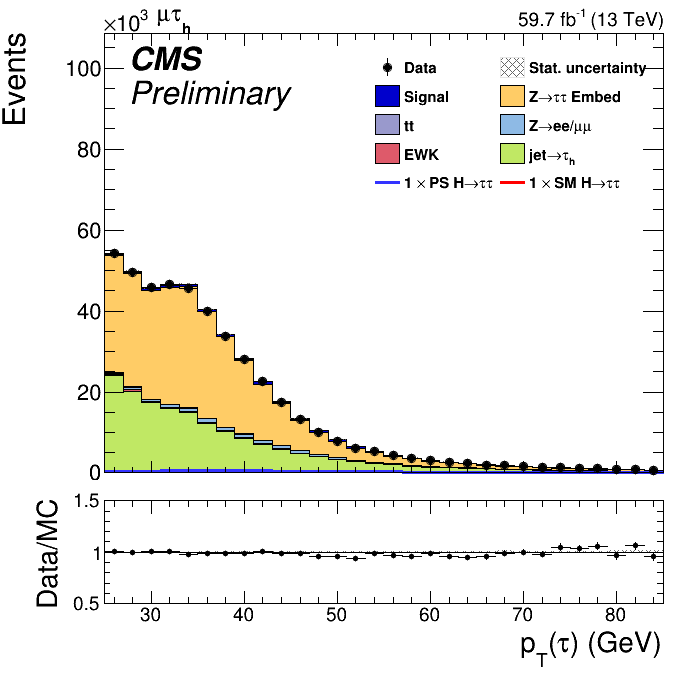
\includegraphics[width=\linewidth]{Chapitre7/Images/CtrlPlots/2018/TaupT.png} 
    \caption{$p^{\tau_h}_T$, 2018.} 
    \vspace{0.5ex}
  \end{subfigure}
  
  \begin{subfigure}[b]{0.33\linewidth}
    \centering
    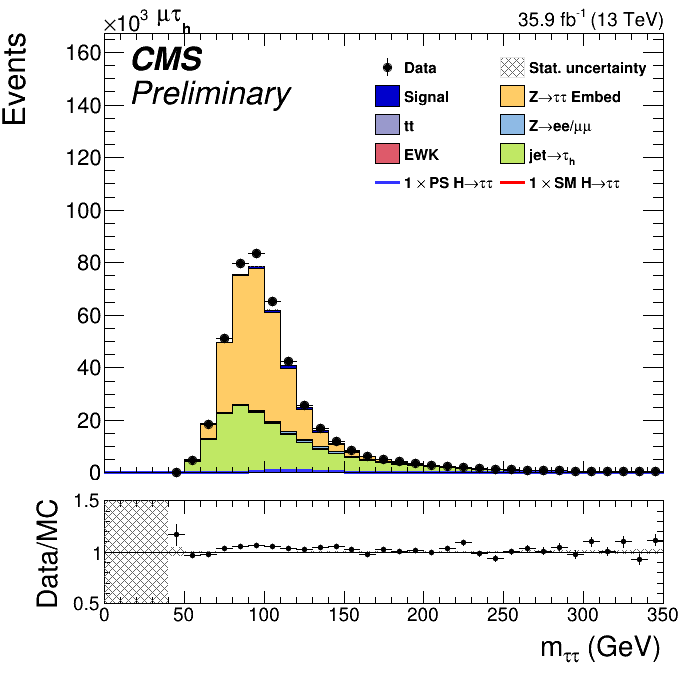
\includegraphics[width=\linewidth]{Chapitre7/Images/CtrlPlots/2016/fastMTTditauMass.png} 
    \caption{Fast MTT $m_{\tau\tau}$, 2016.} 
    \vspace{0.5ex}
  \end{subfigure}%% 
  \begin{subfigure}[b]{0.33\linewidth}
    \centering
    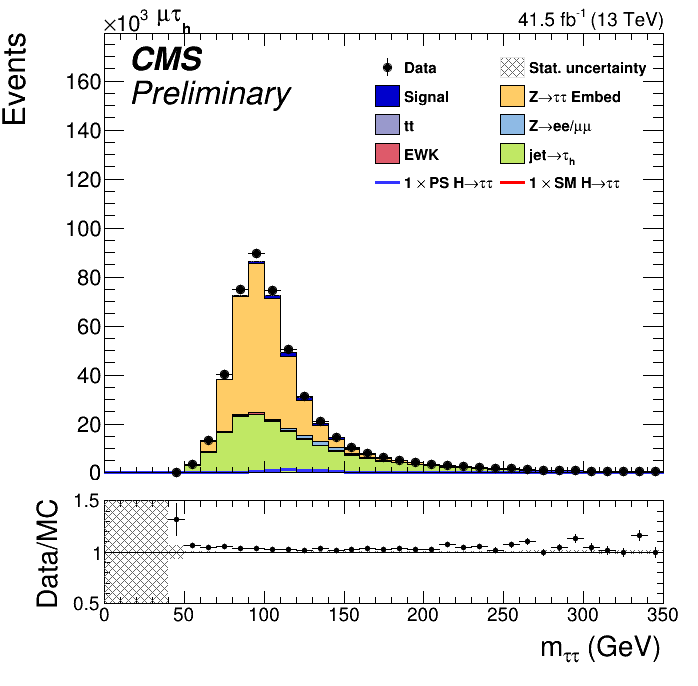
\includegraphics[width=\linewidth]{Chapitre7/Images/CtrlPlots/2017/fastMTTditauMass.png} 
    \caption{Fast MTT $m_{\tau\tau}$, 2017.} 
    \vspace{0.5ex}
  \end{subfigure} 
    \begin{subfigure}[b]{0.33\linewidth}
    \centering
    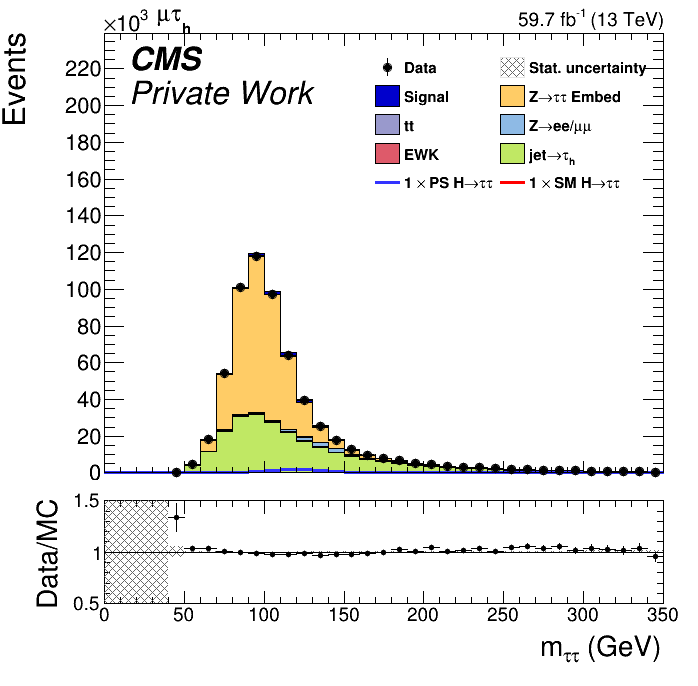
\includegraphics[width=\linewidth]{Chapitre7/Images/CtrlPlots/2018/fastMTTditauMass.png} 
    \caption{Fast MTT $m_{\tau\tau}$, 2018.} 
    \vspace{0.5ex}
  \end{subfigure} 

    \begin{subfigure}[b]{0.33\linewidth}
    \centering
    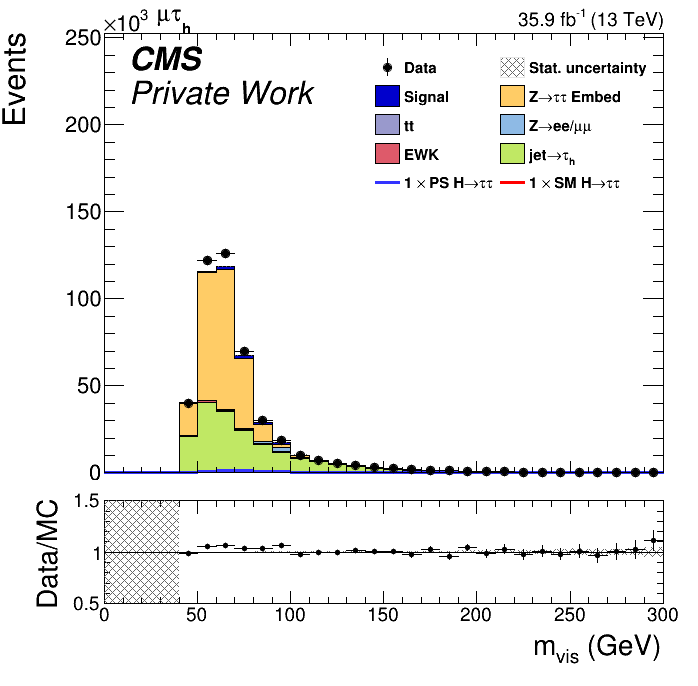
\includegraphics[width=\linewidth]{Chapitre7/Images/CtrlPlots/2016/VisibleMass.png} 
    \caption{$m_{\tau\tau}^{vis}$, 2016.} 
    \vspace{0.5ex}
  \end{subfigure}%% 
  \begin{subfigure}[b]{0.33\linewidth}
    \centering
    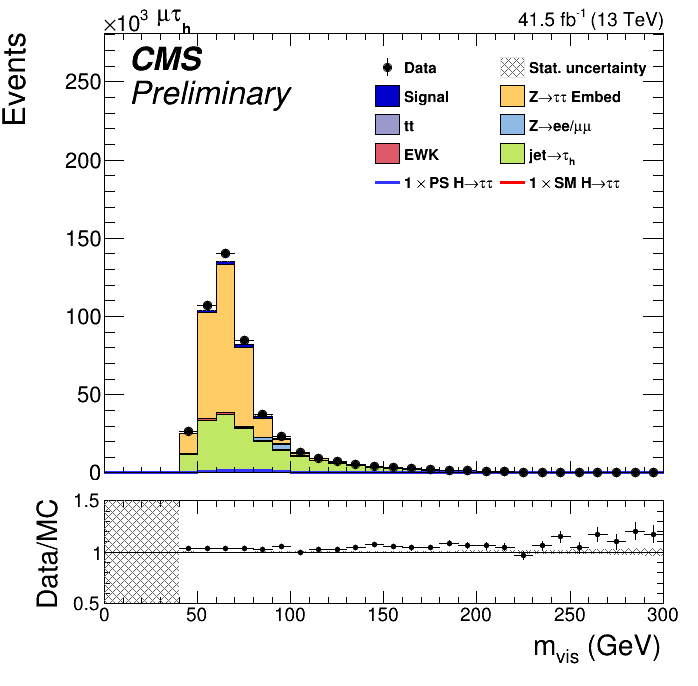
\includegraphics[width=\linewidth]{Chapitre7/Images/CtrlPlots/2017/VisibleMass.png} 
    \caption{$m_{\tau\tau}^{vis}$, 2017.} 
    \vspace{0.5ex}
  \end{subfigure} 
    \begin{subfigure}[b]{0.33\linewidth}
    \centering
    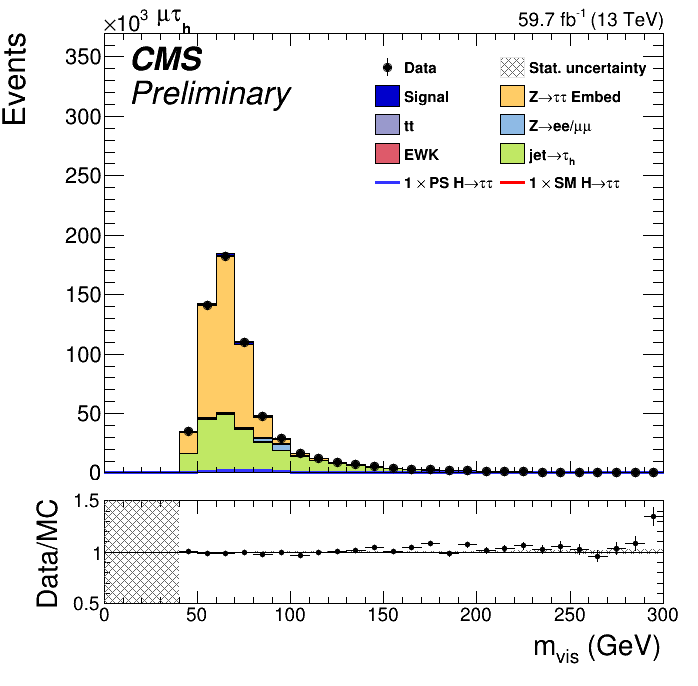
\includegraphics[width=\linewidth]{Chapitre7/Images/CtrlPlots/2018/VisibleMass.png} 
    \caption{$m_{\tau\tau}^{vis}$, 2018.} 
    \vspace{0.5ex}
  \end{subfigure} 
  \caption{}
  \label{page1}
\end{figure}

%page2
\begin{figure}
  \begin{subfigure}[b]{0.33\linewidth}
    \centering
    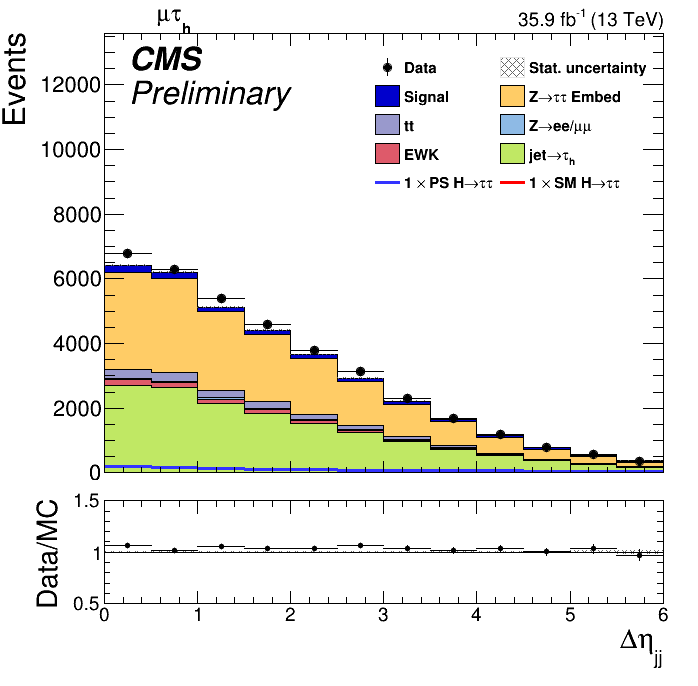
\includegraphics[width=\linewidth]{Chapitre7/Images/CtrlPlots/2016/DijetDeltaEta.png} 
    \caption{$|\Delta\eta|(jj)$, 2016.} 
    \vspace{0.5ex}
  \end{subfigure}%% 
  \begin{subfigure}[b]{0.33\linewidth}
    \centering
    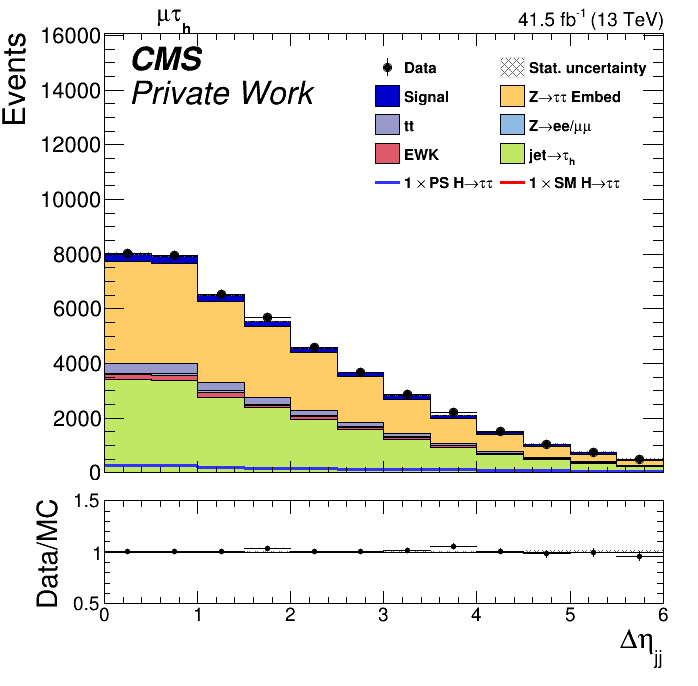
\includegraphics[width=\linewidth]{Chapitre7/Images/CtrlPlots/2017/DijetDeltaEta.png} 
    \caption{$|\Delta\eta|(jj)$, 2017.} 
    \vspace{0.5ex}
  \end{subfigure} 
    \begin{subfigure}[b]{0.33\linewidth}
    \centering
    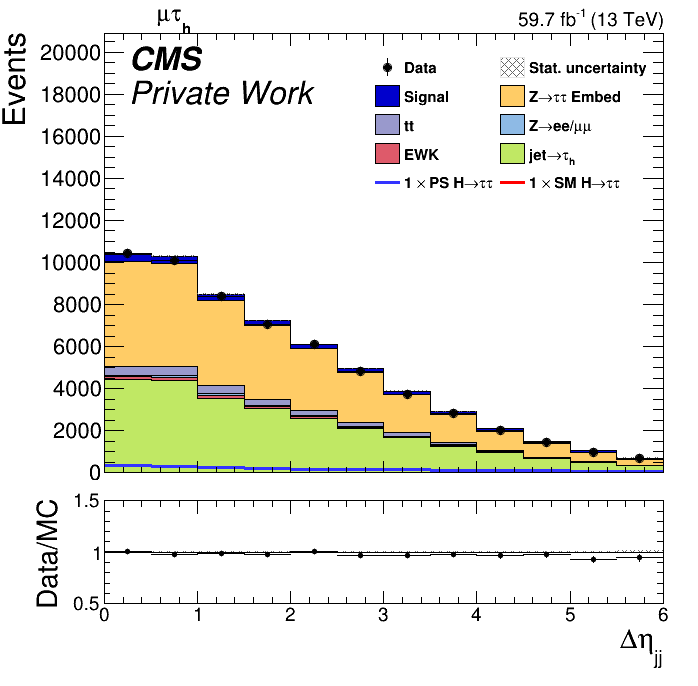
\includegraphics[width=\linewidth]{Chapitre7/Images/CtrlPlots/2018/DijetDeltaEta.png} 
    \caption{$|\Delta\eta|(jj)$, 2018.} 
    \vspace{0.5ex}
  \end{subfigure} 

  \begin{subfigure}[b]{0.33\linewidth}
    \centering
    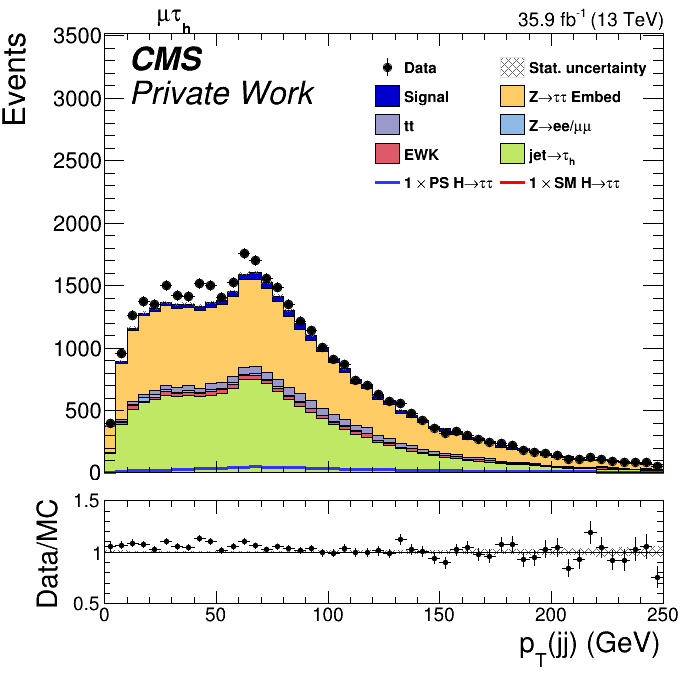
\includegraphics[width=\linewidth]{Chapitre7/Images/CtrlPlots/2016/DijetpT.png} 
    \caption{$p_T(jj)$, 2016.} 
    \vspace{0.5ex}
  \end{subfigure}%% 
  \begin{subfigure}[b]{0.33\linewidth}
    \centering
    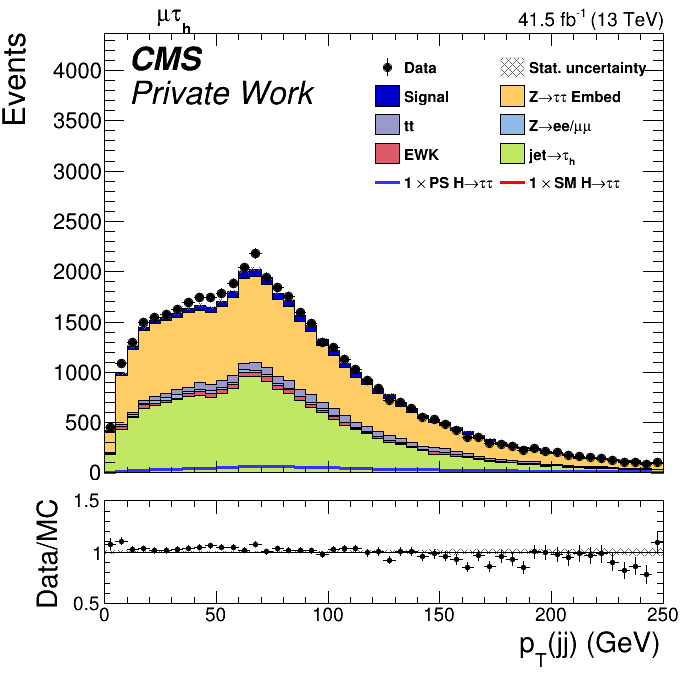
\includegraphics[width=\linewidth]{Chapitre7/Images/CtrlPlots/2017/DijetpT.png} 
    \caption{$p_T(jj)$, 2017.} 
    \vspace{0.5ex}
  \end{subfigure} 
    \begin{subfigure}[b]{0.33\linewidth}
    \centering
    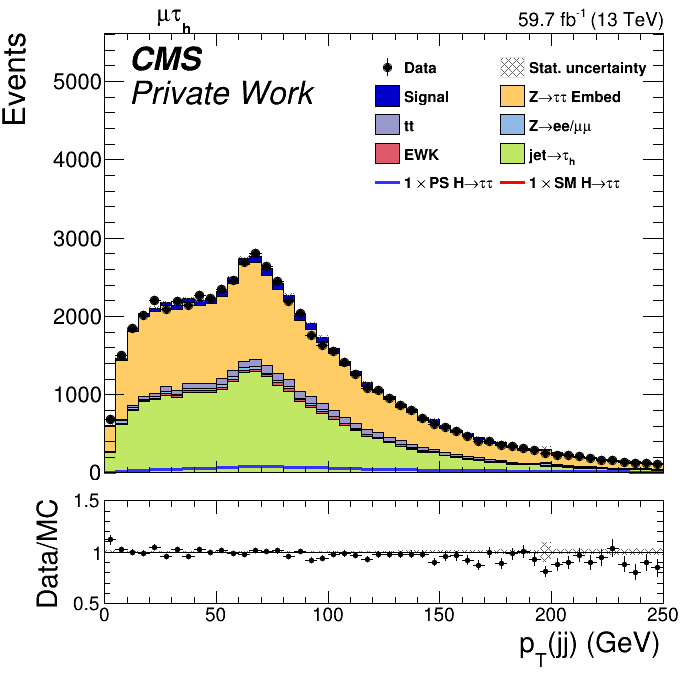
\includegraphics[width=\linewidth]{Chapitre7/Images/CtrlPlots/2018/DijetpT.png} 
    \caption{$p_T(jj)$, 2018.} 
    \vspace{0.5ex}
  \end{subfigure} 

  \begin{subfigure}[b]{0.33\linewidth}
    \centering
    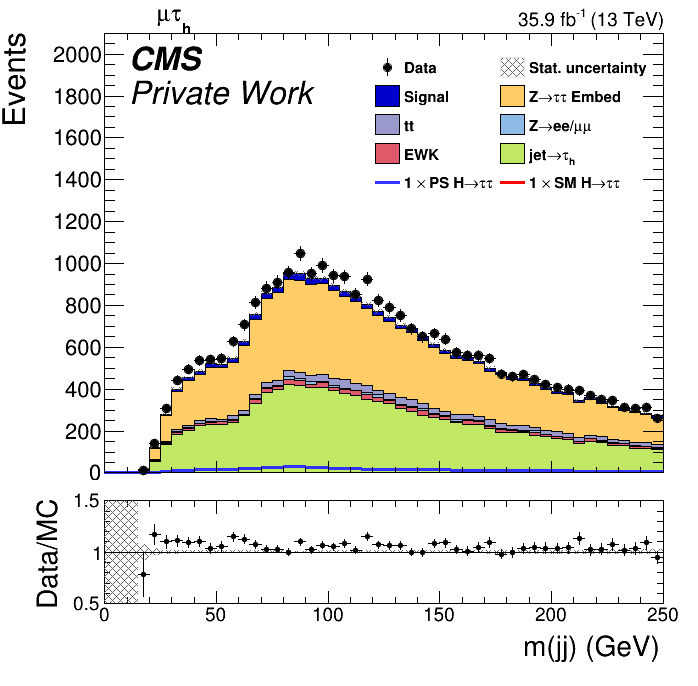
\includegraphics[width=\linewidth]{Chapitre7/Images/CtrlPlots/2016/DijetMass.png} 
    \caption{$m(jj)$, 2016.} 
    \vspace{0.5ex}
  \end{subfigure}%% 
  \begin{subfigure}[b]{0.33\linewidth}
    \centering
    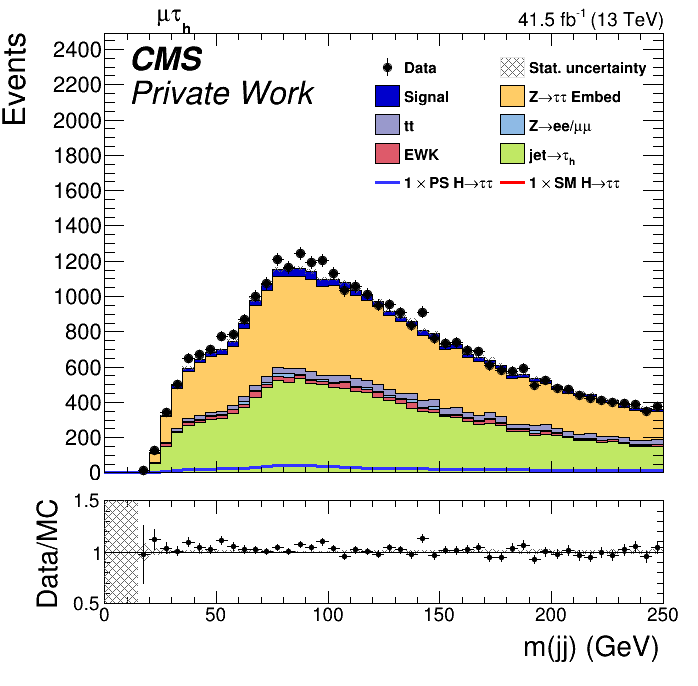
\includegraphics[width=\linewidth]{Chapitre7/Images/CtrlPlots/2017/DijetMass.png} 
    \caption{$m(jj)$, 2017.} 
    \vspace{0.5ex}
  \end{subfigure} 
    \begin{subfigure}[b]{0.33\linewidth}
    \centering
    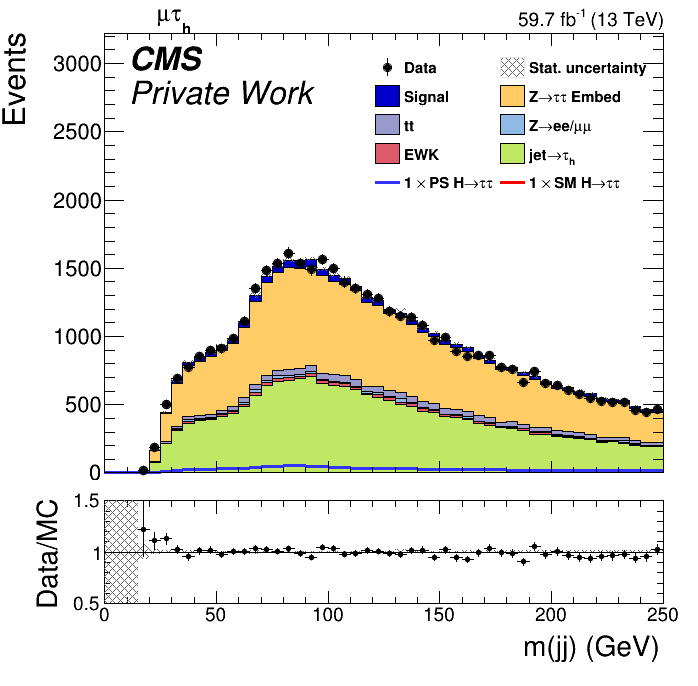
\includegraphics[width=\linewidth]{Chapitre7/Images/CtrlPlots/2018/DijetMass.png} 
    \caption{$m(jj)$, 2018.} 
    \vspace{0.5ex}
  \end{subfigure} 

    \begin{subfigure}[b]{0.33\linewidth}
    \centering
    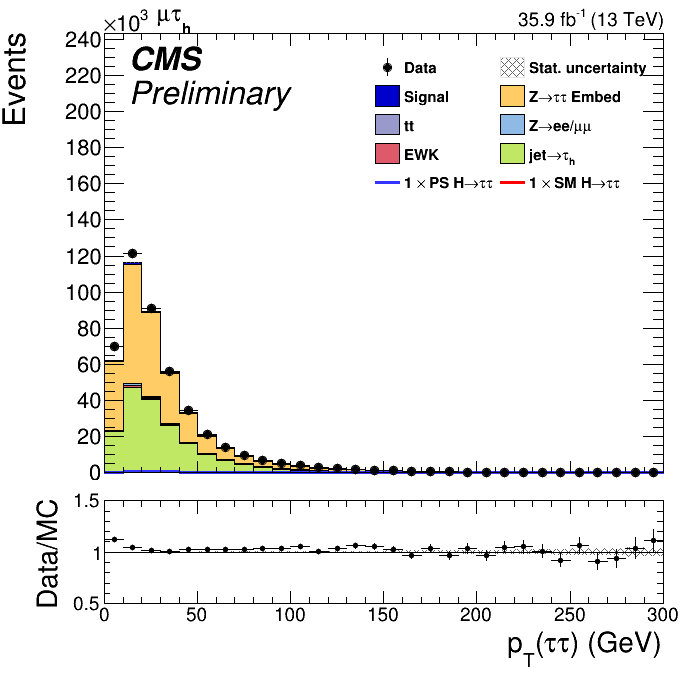
\includegraphics[width=\linewidth]{Chapitre7/Images/CtrlPlots/2016/DitaupT.png} 
    \caption{$p^{\tau\tau}_T$, 2016.} 
    \vspace{0.5ex}
  \end{subfigure}%% 
  \begin{subfigure}[b]{0.33\linewidth}
    \centering
    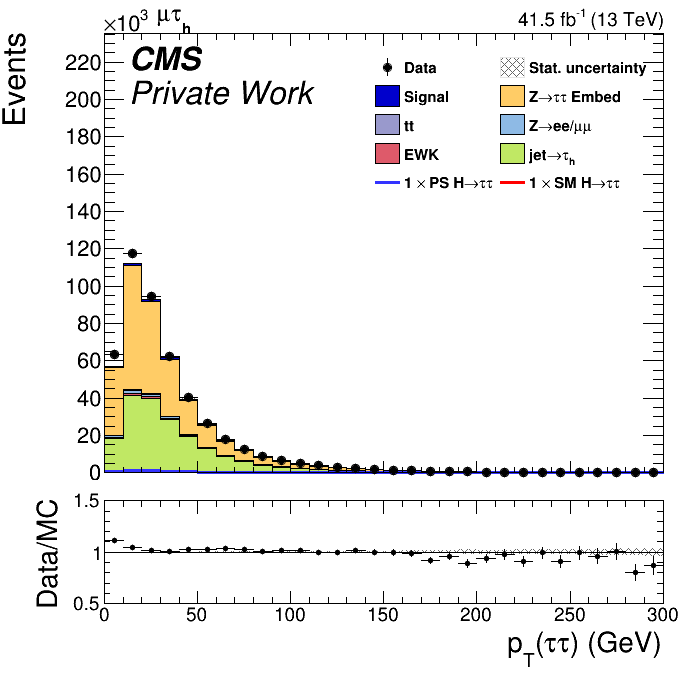
\includegraphics[width=\linewidth]{Chapitre7/Images/CtrlPlots/2017/DitaupT.png} 
    \caption{$p^{\tau\tau}_T$, 2017.} 
    \vspace{0.5ex}
  \end{subfigure} 
    \begin{subfigure}[b]{0.33\linewidth}
    \centering
    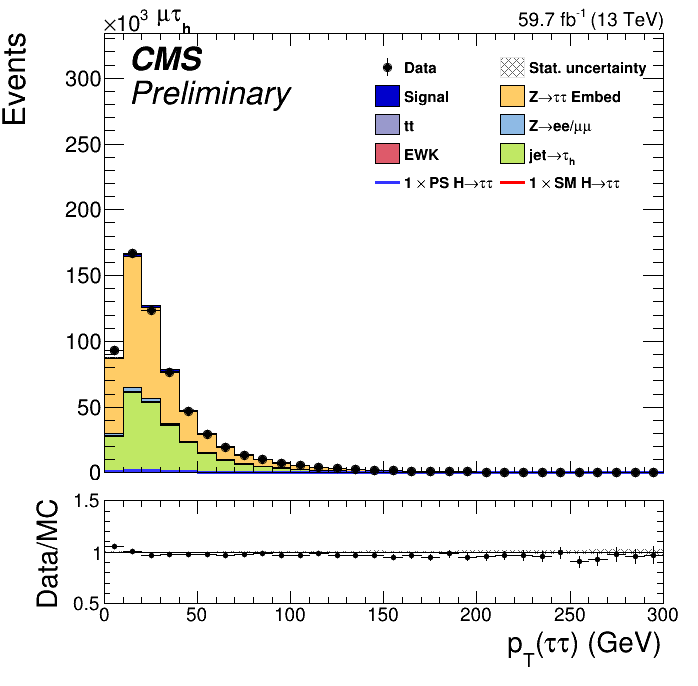
\includegraphics[width=\linewidth]{Chapitre7/Images/CtrlPlots/2018/DitaupT.png} 
    \caption{$p^{\tau\tau}_T$, 2018.} 
    \vspace{0.5ex}
  \end{subfigure} 
  \caption{}
  \label{page2}
\end{figure}

%page3
\begin{figure}
  \begin{subfigure}[b]{0.33\linewidth}
    \centering
    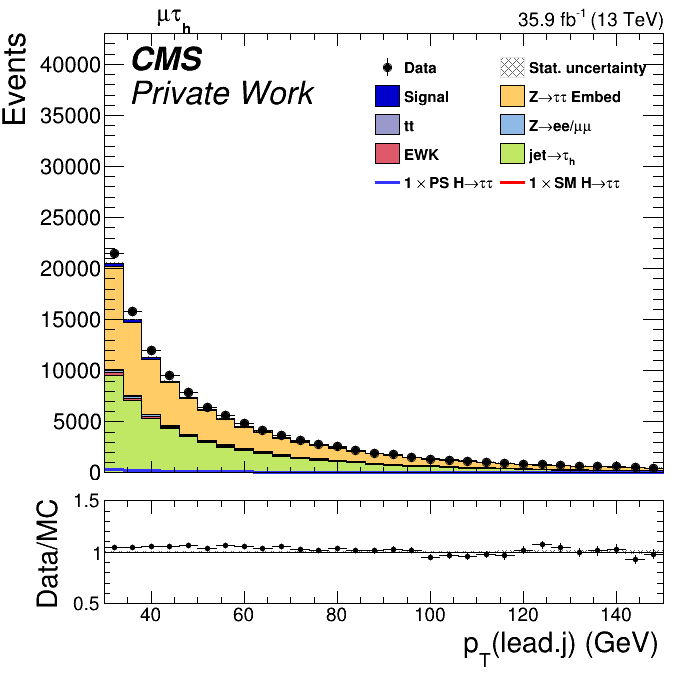
\includegraphics[width=\linewidth]{Chapitre7/Images/CtrlPlots/2016/LeadingJetpT.png} 
    \caption{Leading jet $p_T$, 2016.} 
    \vspace{0.5ex}
  \end{subfigure}%% 
  \begin{subfigure}[b]{0.33\linewidth}
    \centering
    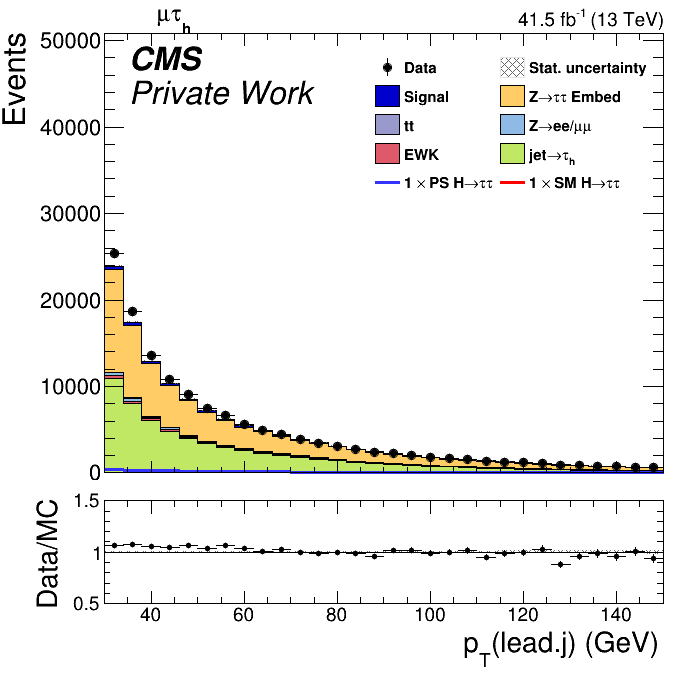
\includegraphics[width=\linewidth]{Chapitre7/Images/CtrlPlots/2017/LeadingJetpT.png} 
    \caption{Leading jet $p_T$, 2017.} 
    \vspace{0.5ex}
  \end{subfigure} 
    \begin{subfigure}[b]{0.33\linewidth}
    \centering
    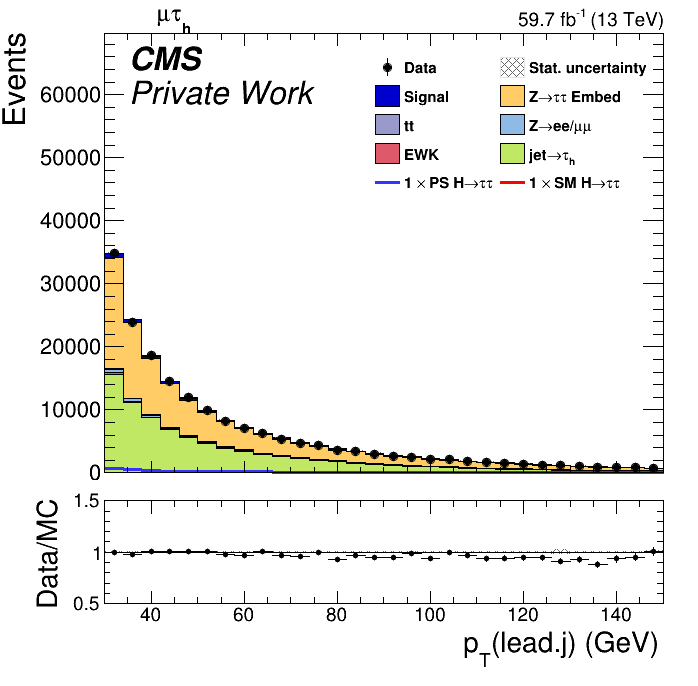
\includegraphics[width=\linewidth]{Chapitre7/Images/CtrlPlots/2018/LeadingJetpT.png} 
    \caption{Leading jet $p_T$, 2018.} 
    \vspace{0.5ex}
  \end{subfigure} 

    \begin{subfigure}[b]{0.33\linewidth}
    \centering
    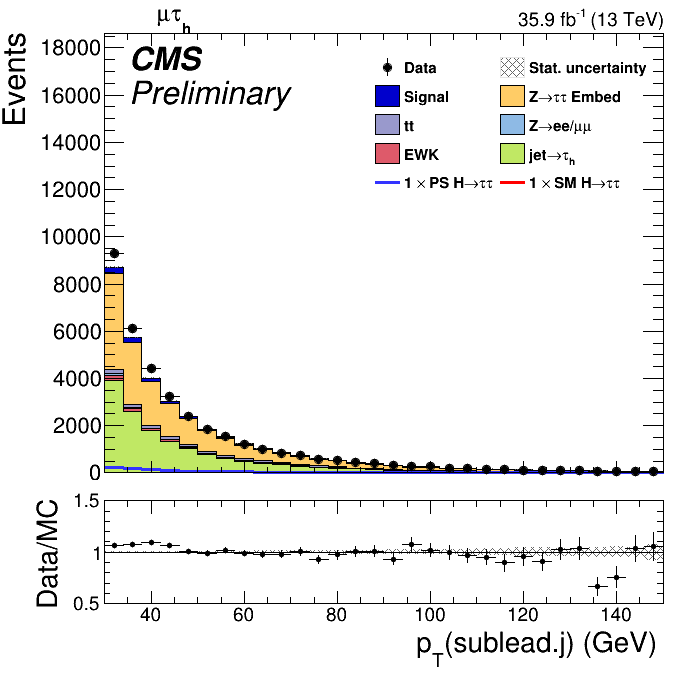
\includegraphics[width=\linewidth]{Chapitre7/Images/CtrlPlots/2016/SubleadingJetpT.png} 
    \caption{Subleading jet $p_T$, 2016.} 
    \vspace{0.5ex}
  \end{subfigure}%% 
  \begin{subfigure}[b]{0.33\linewidth}
    \centering
    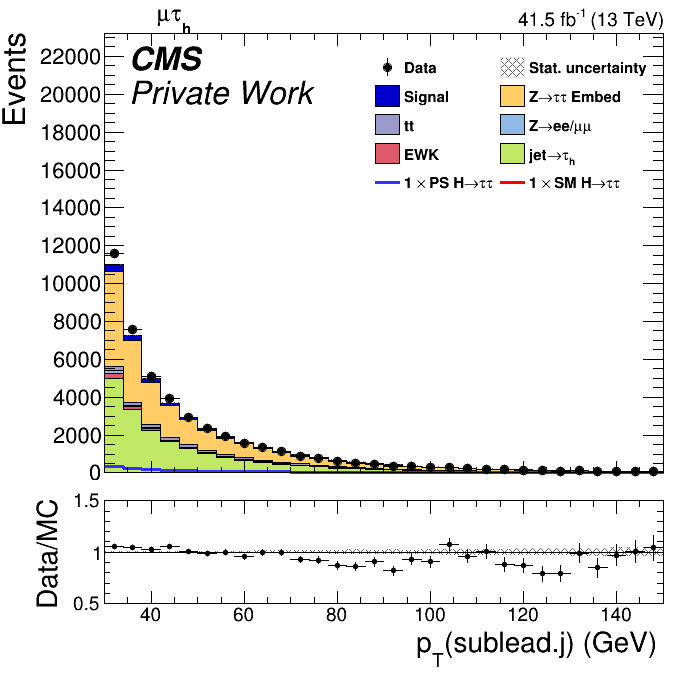
\includegraphics[width=\linewidth]{Chapitre7/Images/CtrlPlots/2017/SubleadingJetpT.png} 
    \caption{Subleading jet $p_T$, 2017.} 
    \vspace{0.5ex}
  \end{subfigure} 
    \begin{subfigure}[b]{0.33\linewidth}
    \centering
    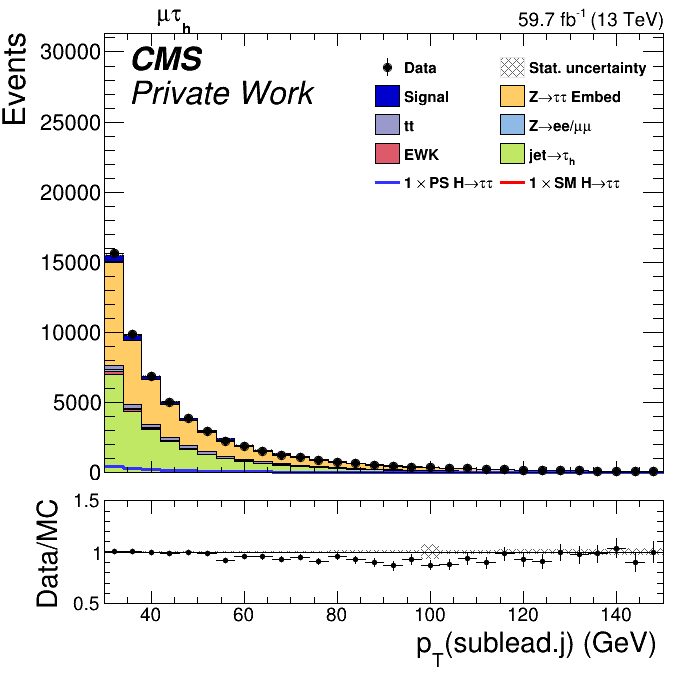
\includegraphics[width=\linewidth]{Chapitre7/Images/CtrlPlots/2018/SubleadingJetpT.png} 
    \caption{Subleading jet $p_T$, 2018.} 
    \vspace{0.5ex}
  \end{subfigure}
  
  \begin{subfigure}[b]{0.33\linewidth}
    \centering
    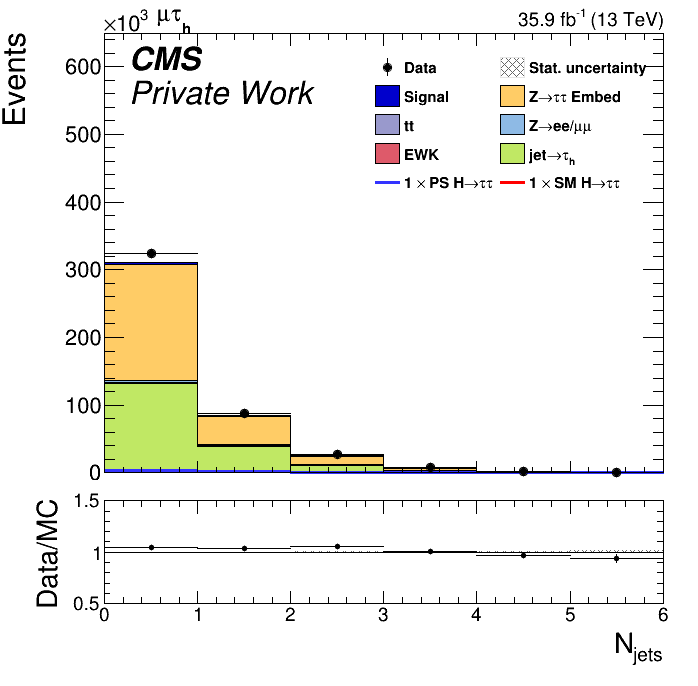
\includegraphics[width=\linewidth]{Chapitre7/Images/CtrlPlots/2016/Njets.png} 
    \caption{$N$ jets, 2016.} 
    \vspace{0.5ex}
  \end{subfigure}%% 
  \begin{subfigure}[b]{0.33\linewidth}
    \centering
    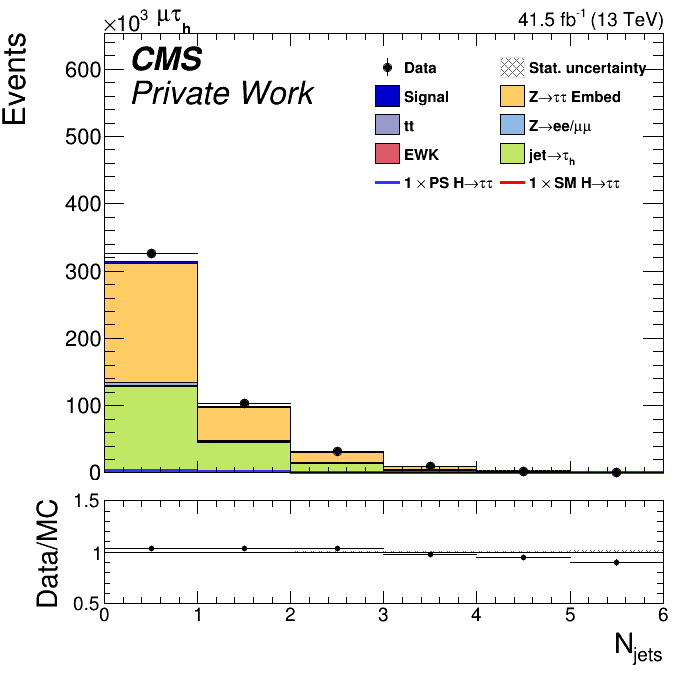
\includegraphics[width=\linewidth]{Chapitre7/Images/CtrlPlots/2017/Njets.png} 
    \caption{$N$ jets, 2017.} 
    \vspace{0.5ex}
  \end{subfigure} 
    \begin{subfigure}[b]{0.33\linewidth}
    \centering
    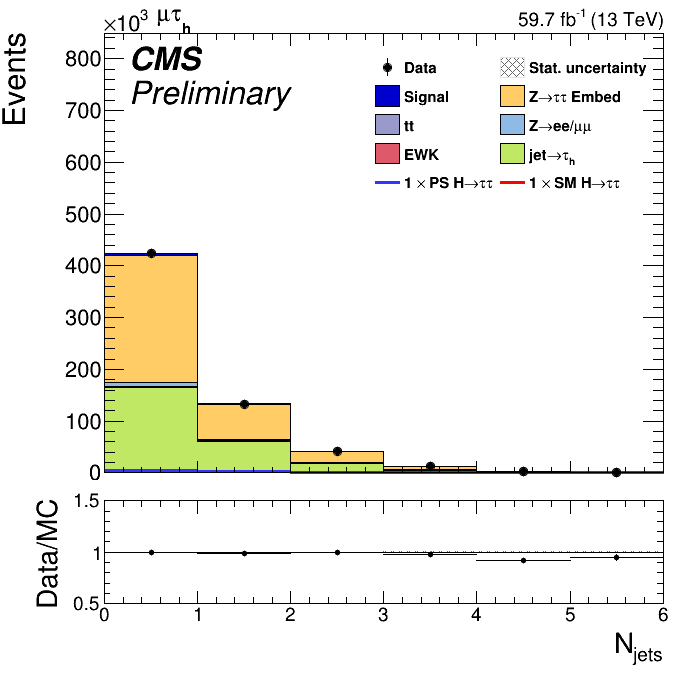
\includegraphics[width=\linewidth]{Chapitre7/Images/CtrlPlots/2018/Njets.png} 
    \caption{$N$ jets, 2018.} 
    \vspace{0.5ex}
  \end{subfigure} 

    \begin{subfigure}[b]{0.33\linewidth}
    \centering
    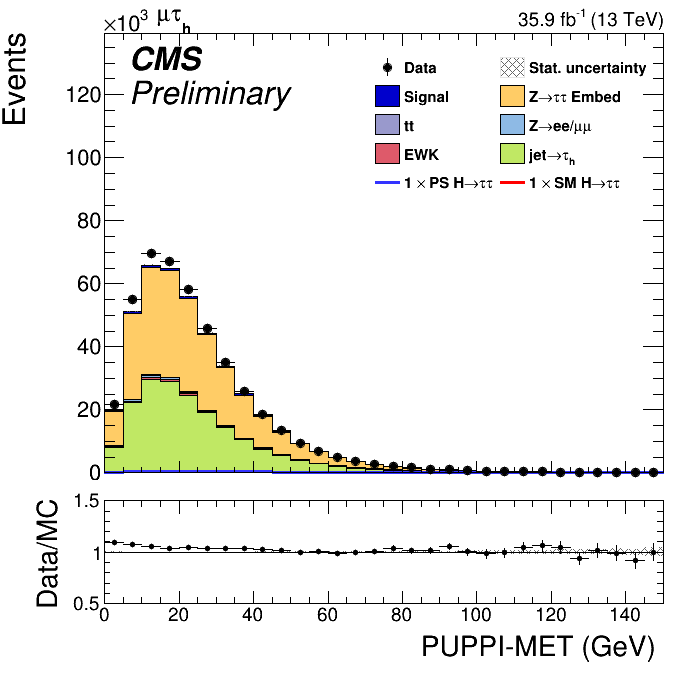
\includegraphics[width=\linewidth]{Chapitre7/Images/CtrlPlots/2016/PUPPImet.png} 
    \caption{$p^{mis}_T$, 2016.} 
    \vspace{0.5ex}
  \end{subfigure}%% 
  \begin{subfigure}[b]{0.33\linewidth}
    \centering
    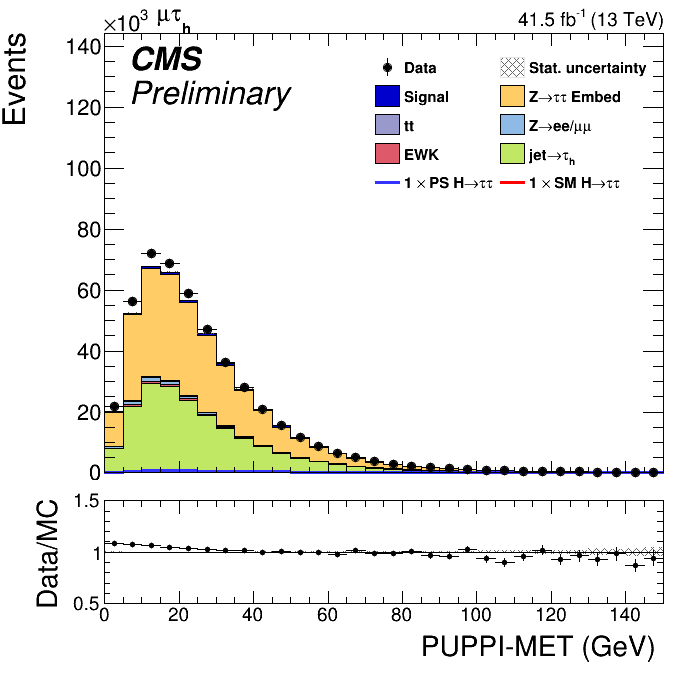
\includegraphics[width=\linewidth]{Chapitre7/Images/CtrlPlots/2017/PUPPImet.png} 
    \caption{$p^{mis}_T$, 2017.} 
    \vspace{0.5ex}
  \end{subfigure} 
    \begin{subfigure}[b]{0.33\linewidth}
    \centering
    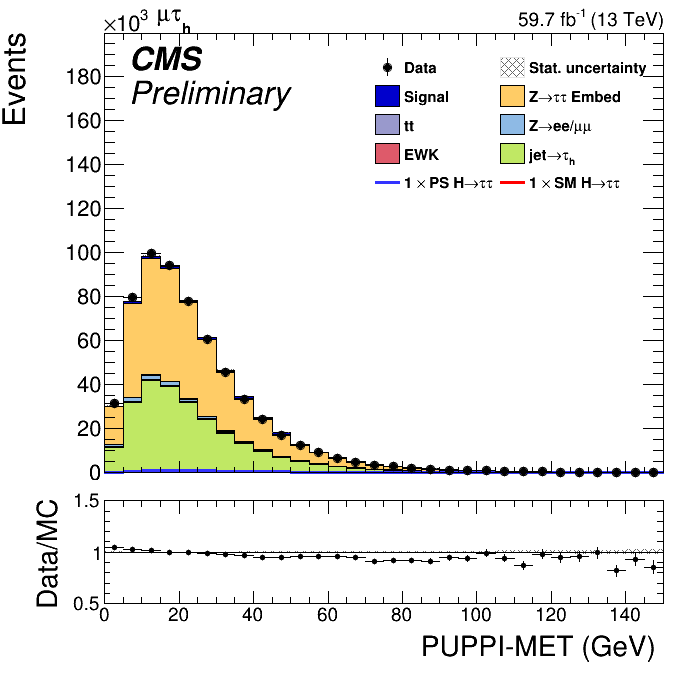
\includegraphics[width=\linewidth]{Chapitre7/Images/CtrlPlots/2018/PUPPImet.png} 
    \caption{$p^{mis}_T$, 2018.} 
    \vspace{0.5ex}
  \end{subfigure} 
  \caption{}
  \label{page3}
\end{figure}

\begin{figure}
    \begin{subfigure}[b]{0.33\linewidth}
    \centering
    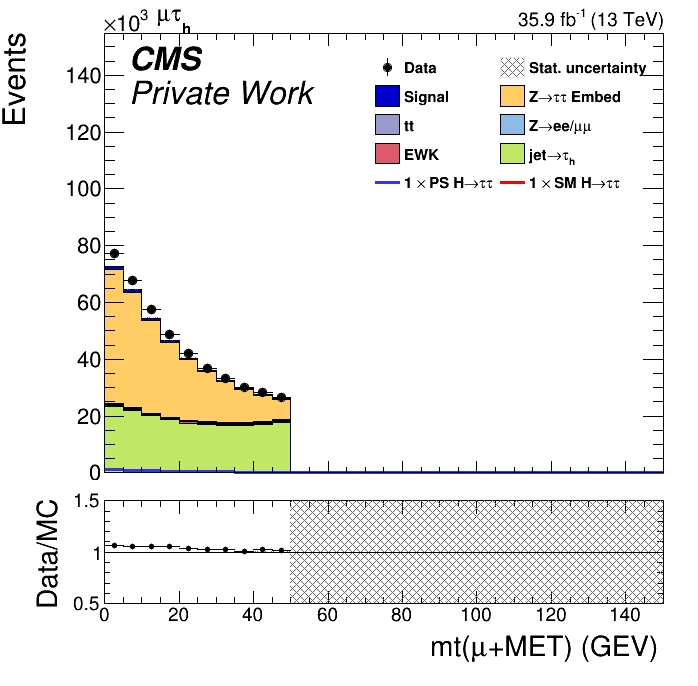
\includegraphics[width=\linewidth]{Chapitre7/Images/CtrlPlots/2016/MuMETmt.png} 
    \caption{$m^{\mu+MET}_T$, 2016.} 
    \vspace{0.5ex}
  \end{subfigure}%% 
  \begin{subfigure}[b]{0.33\linewidth}
    \centering
    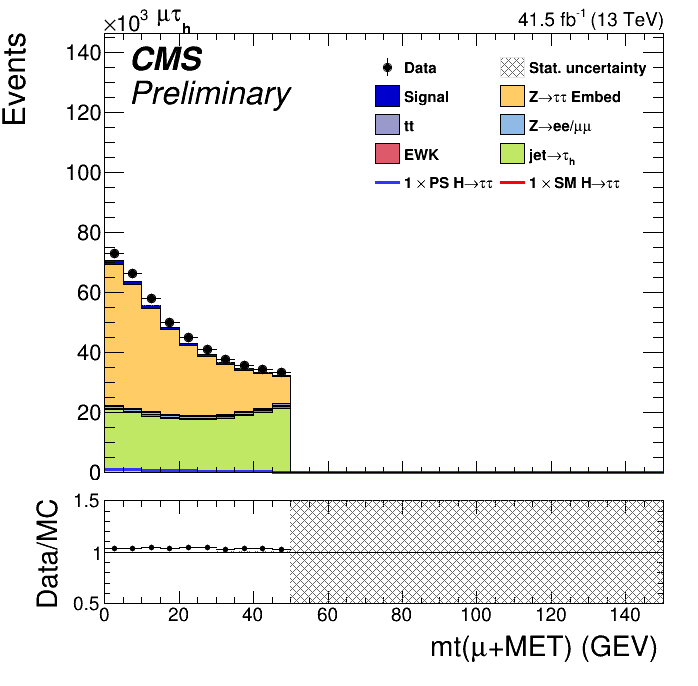
\includegraphics[width=\linewidth]{Chapitre7/Images/CtrlPlots/2017/MuMETmt.png} 
    \caption{$m^{\mu+MET}_T$, 2017.} 
    \vspace{0.5ex}
  \end{subfigure} 
    \begin{subfigure}[b]{0.33\linewidth}
    \centering
    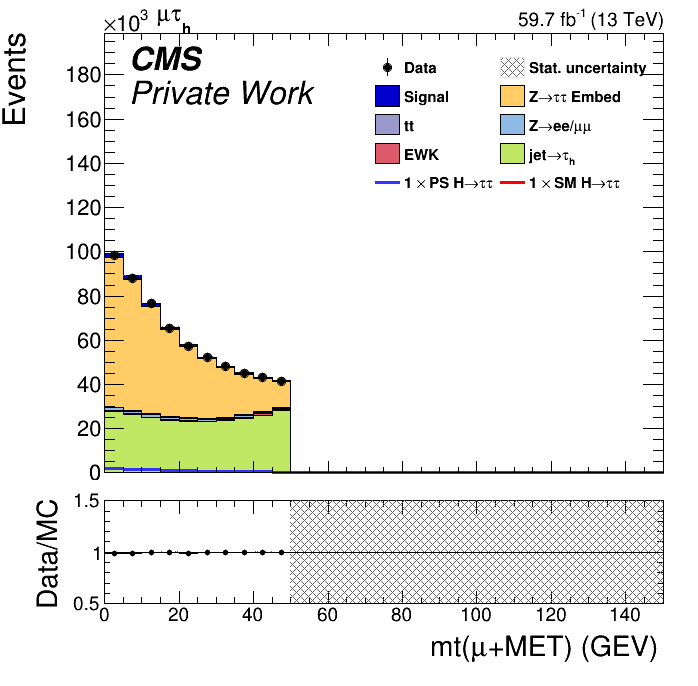
\includegraphics[width=\linewidth]{Chapitre7/Images/CtrlPlots/2018/MuMETmt.png} 
    \caption{$m^{\mu+MET}_T$, 2018.} 
    \vspace{0.5ex}
  \end{subfigure} 
  \caption{}
  \label{page4}
\end{figure}

Distribution du score de sortie du BDT dans la catégorie Jet Fakes (a), $Z\rightarrow\tau\tau$ Embed (b) et Higgs (c) pour les données de 2018. Les données sont masquées dans la troisième catégorie dans laquelle le signal est attendu.

\begin{figure}[!ht]
    \begin{subfigure}[b]{0.33\linewidth}
    \centering
    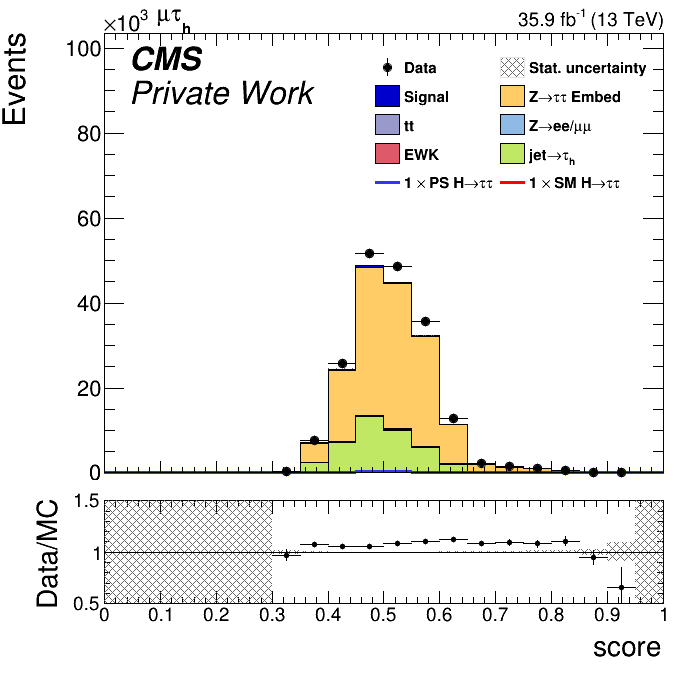
\includegraphics[width=\linewidth]{Chapitre7/Images/CtrlPlots/2016/BDTscoreZTT.png} 
    \caption{$Z\to\tau\tau$, 2016.} 
    \vspace{0.5cm}
  \end{subfigure}%% 
  \begin{subfigure}[b]{0.33\linewidth}
    \centering
    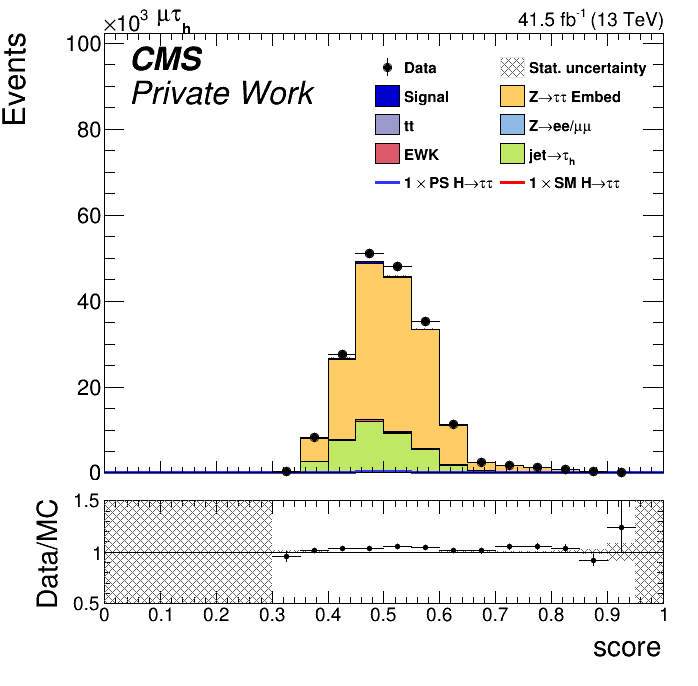
\includegraphics[width=\linewidth]{Chapitre7/Images/CtrlPlots/2017/BDTscoreZTT.png} 
    \caption{$Z\to\tau\tau$, 2017.} 
    \vspace{0.5cm}
  \end{subfigure} 
    \begin{subfigure}[b]{0.33\linewidth}
    \centering
    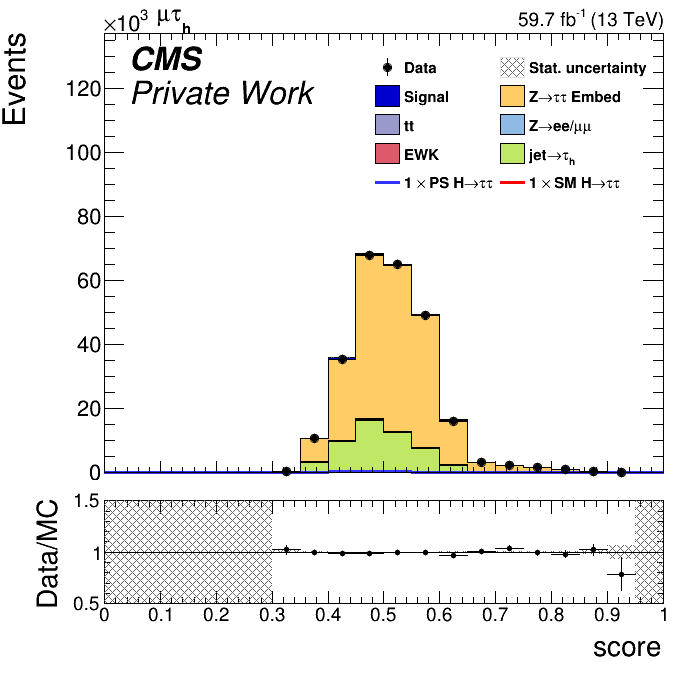
\includegraphics[width=\linewidth]{Chapitre7/Images/CtrlPlots/2018/BDTscoreZTT.png} 
    \caption{$Z\to\tau\tau$, 2018.} 
    \vspace{0.5cm}
  \end{subfigure} 
  %%
  \begin{subfigure}[b]{0.33\linewidth}
    \centering
    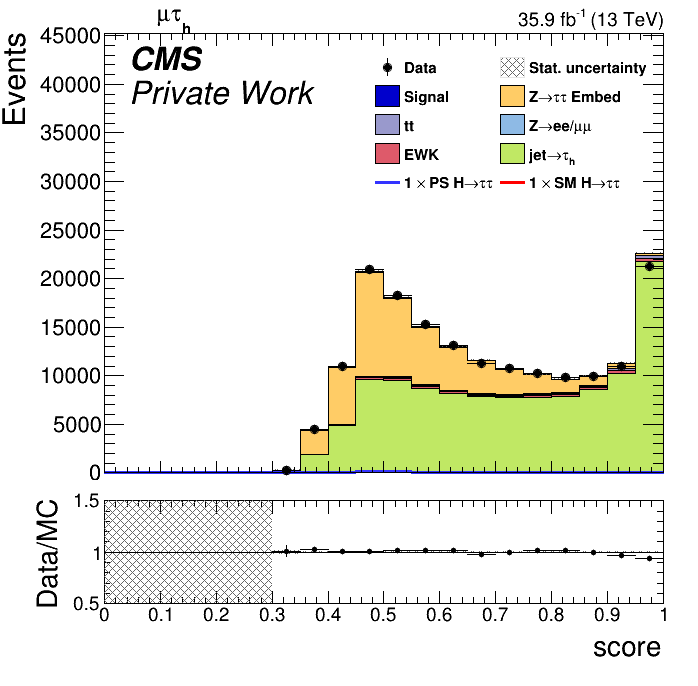
\includegraphics[width=\linewidth]{Chapitre7/Images/CtrlPlots/2016/BDTscoreJetFakes.png} 
    \caption{JetFakes, 2016.} 
    \vspace{0.5cm}
  \end{subfigure}%% 
  \begin{subfigure}[b]{0.33\linewidth}
    \centering
    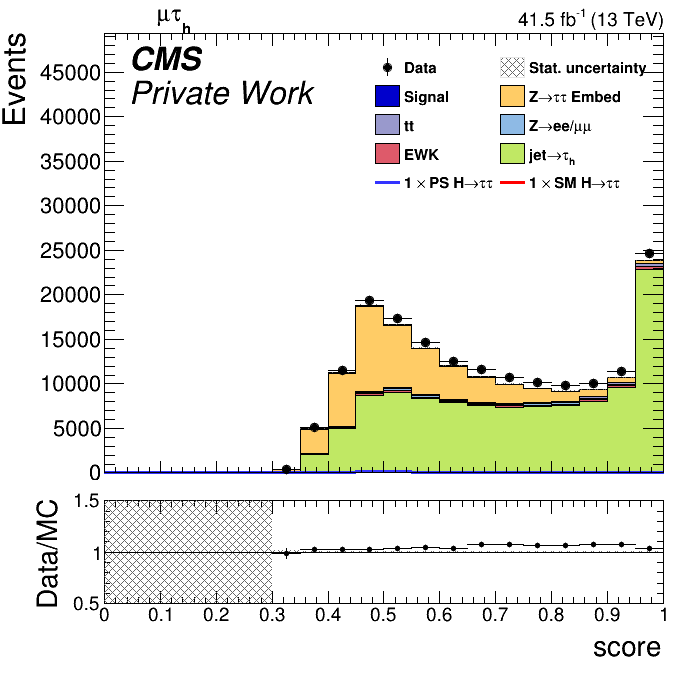
\includegraphics[width=\linewidth]{Chapitre7/Images/CtrlPlots/2017/BDTscoreJetFakes.png} 
    \caption{JetFakes, 2017.} 
    \vspace{0.5cm}
  \end{subfigure} 
    \begin{subfigure}[b]{0.33\linewidth}
    \centering
    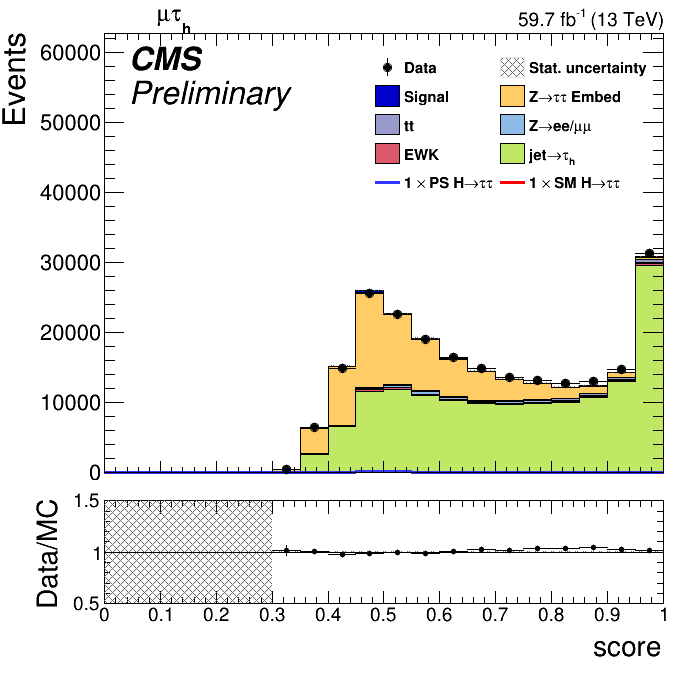
\includegraphics[width=\linewidth]{Chapitre7/Images/CtrlPlots/2018/BDTscoreJetFakes.png} 
    \caption{JetFakes, 2018.} 
    \vspace{0.5cm}
  \end{subfigure} 
  %%
  \begin{subfigure}[b]{0.33\linewidth}
    \centering
    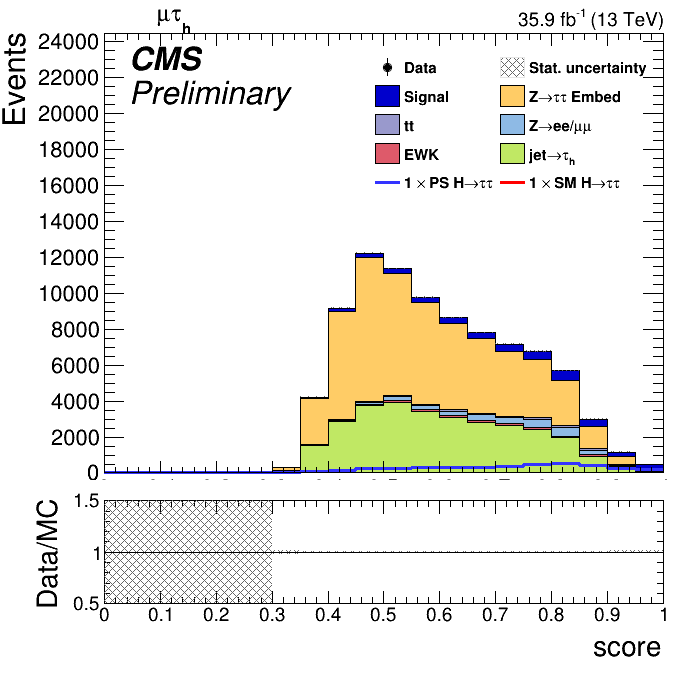
\includegraphics[width=\linewidth]{Chapitre7/Images/CtrlPlots/2016/BDTscoreHiggs.png} 
    \caption{Higgs, 2016.} 
    \vspace{0.5ex}
  \end{subfigure}%% 
  \begin{subfigure}[b]{0.33\linewidth}
    \centering
    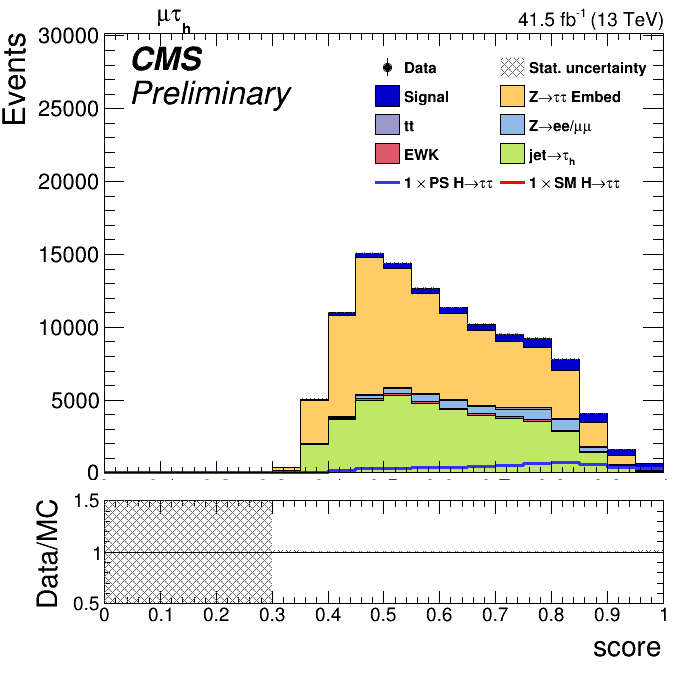
\includegraphics[width=\linewidth]{Chapitre7/Images/CtrlPlots/2017/BDTscoreHiggs.png} 
    \caption{Higgs, 2017.} 
    \vspace{0.5ex}
  \end{subfigure} 
    \begin{subfigure}[b]{0.33\linewidth}
    \centering
    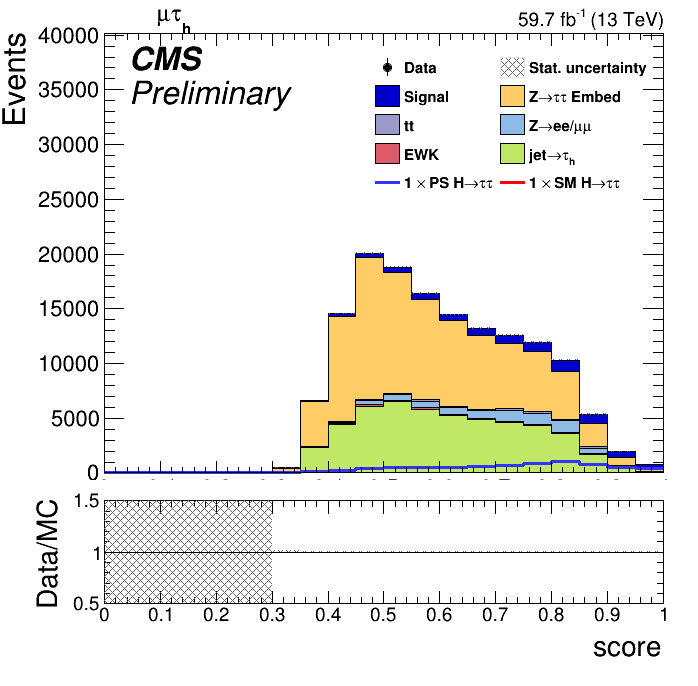
\includegraphics[width=\linewidth]{Chapitre7/Images/CtrlPlots/2018/BDTscoreHiggs.png} 
    \caption{Higgs, 2018.} 
    \vspace{0.5ex}
  \end{subfigure} 
  \caption{Distribution du score de sortie du BDT dans la catégorie $Z\to\tau\tau$ (haut), \textit{jetFakes} (milieu) et Higgs (bas) pour les données de 2016, 0271 et 2018. Les données sont masquées dans la troisième catégorie dans laquelle le signal est attendu.}
  \label{BDTscores}
\end{figure}